\documentclass[10pt,twocolumn,a4paper]{article}

\usepackage[a4paper,top=1.7cm,bottom=1.8cm,left=1.6cm,right=1.6cm,columnsep=0.6cm]{geometry}
\usepackage[T1]{fontenc}
\usepackage{mathptmx}
\usepackage{courier}  % Type 1 typewriter font
\usepackage{microtype}
\usepackage{amsmath}
\usepackage{booktabs}
\usepackage{graphicx}
\usepackage[font=small,labelfont=bf,skip=4pt]{caption}
\usepackage[numbers,sort&compress]{natbib}
\usepackage[hidelinks]{hyperref}
\hypersetup{pdftitle={Can We Trust an Ablation Study? Silent Errors and Seed Variance in Two Incremental NLP Studies}, pdfauthor={Andrea Giampietro}}

\makeatletter
\renewcommand\section{\@startsection{section}{1}{\z@}{-7pt plus -2pt minus -1pt}{3pt}%
  {\normalfont\normalsize\bfseries}}
\renewcommand\subsection{\@startsection{subsection}{2}{\z@}{-5pt plus -1pt minus -1pt}{2pt}%
  {\normalfont\normalsize\bfseries\itshape}}
\makeatother
\newenvironment{tightlist}{\begin{itemize}\setlength{\itemsep}{1pt}\setlength{\parskip}{0pt}%
  \setlength{\topsep}{2pt}\setlength{\leftmargin}{1.1em}}{\end{itemize}}
\newcommand{\para}[1]{\textbf{#1}\hspace{0.4em}}
\setlength{\textfloatsep}{8pt plus 2pt minus 2pt}
\setlength{\dbltextfloatsep}{8pt plus 2pt minus 2pt}

\begin{document}

\twocolumn[
\begin{center}
  {\Large\bfseries Can We Trust an Ablation Study?\\[2pt]
  Silent Errors and Seed Variance in Two Incremental NLP Studies\par}
  \vspace{8pt}
  {\normalsize Andrea Giampietro\par}
  \vspace{2pt}
  {\small University of Trento\par}
  {\small\url{https://github.com/giampyhatesyou/Natural_Language_Processing}\par}
  \vspace{8pt}
  \begin{minipage}{0.86\textwidth}
  \small\noindent\textbf{Abstract.}
  Ablation studies are the main evidence that a technique helps, yet their conclusions rest on code that is
  rarely tested. We audit an incremental ablation study of two classic NLP tasks, word-level language modelling
  on the Penn Treebank (an LSTM improved with dropout, AdamW, weight tying, variational dropout and NT-AvSGD) and
  joint intent classification and slot filling on ATIS (LSTM, BiLSTM, dropout, BERT), and compare the effects it
  reported with those of a re-implementation verified by tests. Of the ten step-wise effects, seven change: two
  reverse sign, three are off by more than a factor of two, and the two gains of dropout on ATIS are within the
  variation between seeds. None of the errors behind these changes raised an exception or produced an implausible
  number, and two were explained away in the original report. Re-introduced one at a time as mutants, the audited
  errors and three plausible variants of them, sixteen in all, are caught by a suite of behavioural, oracle and
  invariance tests that runs in under a minute on a CPU. We argue that every ablation step should come with a configuration diff, a confidence interval and a
  test that fails if the technique is silently disabled.
  \end{minipage}
  \vspace{12pt}
\end{center}
]

\section{Introduction}

\begin{figure*}[t]
  \centering
  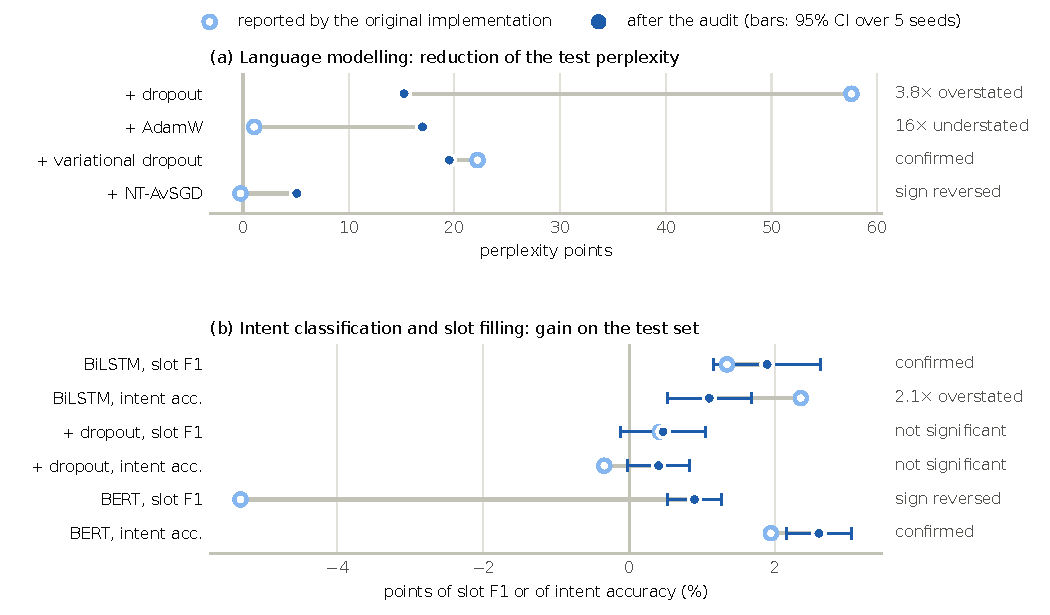
\includegraphics[width=0.86\textwidth]{figures/effects.pdf}
  \caption{Effect of each ablation step as reported by the original implementation (hollow) and after the audit
  (filled; bars: 95\% CI of the difference over 5 seeds, language models trained once). Right of zero, the step
  helps. The label on the right is the outcome of the comparison (Section~\ref{sec:audit}).}
  \label{fig:effects}
\end{figure*}

An ablation study adds or removes one component at a time and attributes the change in a metric to that
component. Its conclusions are only as reliable as two assumptions: that the code implements what the paper
describes, and that the measured differences exceed the variation between runs. The second assumption has been
studied extensively in NLP: scores of the same model vary across seeds enough to reorder methods
\cite{reimers2017distributions,melis2018evaluation,bouthillier2021variance}, and significance testing is often
missing or misapplied \cite{dror2018hitchhiker,dodge2019showyourwork}. The first is harder to study, because
implementation errors are invisible once the numbers are published \cite{sculley2015debt,lipton2019troubling}.

This paper studies both assumptions on a case where two implementations of the same study exist. The study
improves two models step by step: an LSTM language model on the Penn Treebank and a joint intent and slot model on
ATIS. Its original implementation was the author's final project for the Natural Language Understanding course of
the University of Trento (2025); a later audit found errors in it and replaced it with a re-implementation
whose algorithms and evaluation are covered by tests. We ask three questions:
\begin{tightlist}
  \item \textbf{RQ1.} How much did the errors change the conclusions of the study?
  \item \textbf{RQ2.} Once the errors are fixed, which effects survive the variation between seeds?
  \item \textbf{RQ3.} Which checks catch the errors, and at what cost?
\end{tightlist}
Seven of the ten step-wise effects changed (Figure~\ref{fig:effects}), every error was silent, and all of them are
caught by tests that a reviewer could ask for. Code, per-run results and tests are public.

\section{Related work}

\para{Variance and significance.} Reimers and Gurevych \cite{reimers2017distributions} show that the random seed
alone changes the scores of LSTM sequence taggers enough to change which system looks best, and recommend
reporting score distributions. Dror et
al.~\cite{dror2018hitchhiker} survey how rarely NLP papers test significance, Dodge et
al.~\cite{dodge2019showyourwork} tie conclusions to the tuning budget, and Bouthillier et
al.~\cite{bouthillier2021variance} quantify the sources of variance in benchmarks. Melis et
al.~\cite{melis2018evaluation} find that well-tuned LSTM language models beat more recent architectures, a warning
that weak baselines inflate gains.

\para{Errors in ML code.} Sculley et al.~\cite{sculley2015debt} describe the technical debt that accumulates in
ML systems, and Lipton and Steinhardt \cite{lipton2019troubling} list the failure to identify the source of
empirical gains among the troubling trends of the field. Reproducibility programmes \cite{pineau2021reproducibility}
ask for code and experimental details; the correctness of that code is left to the authors. Mutation testing \cite{demillo1978hints,jia2011mutation} measures a test suite by injecting faults
and counting how many it detects; we use it with faults taken from a real audit.

\section{Case studies and protocol}

\para{Language modelling.} Penn Treebank \cite{marcus1993ptb} in the preprocessing of Mikolov et
al.~\cite{mikolov2010rnnlm}: 42,068 / 3,370 / 3,761 sentences, a 10k-word vocabulary, one sentence per sample with
an end-of-sentence token, padding excluded from the loss. All models have 256-dimensional embeddings and one LSTM
layer \cite{hochreiter1997lstm} of 256 units. Part~A adds dropout \cite{srivastava2014dropout} ($p=0.4$ on the
embeddings and on the LSTM outputs) to the LSTM trained with SGD (lr 2, batch 64), then replaces SGD with AdamW
\cite{loshchilov2019adamw} (lr $10^{-3}$, weight decay 0.01). Part~B follows AWD-LSTM \cite{merity2018awdlstm} with
plain SGD (lr 1.5, batch 32): weight tying \cite{press2017tying,inan2017tying}, then variational dropout
\cite{gal2016dropout} (one mask per sequence), then NT-AvSGD, which averages the iterates \cite{polyak1992averaging}
once the dev perplexity $v$ of epoch $t$ satisfies $t>n$ and $v>\min_{i\le t-n} v_i$ ($n=5$). Training stops after 3
epochs without dev improvement; with NT-AvSGD there is no early stopping before the trigger and a patience of 5,
measured on the averaged weights, after it. Metric: perplexity (PPL).

\para{Intent classification and slot filling.} ATIS \cite{hemphill1990atis}: 4,978 training and 893 test
utterances, 26 intents, 129 IOB slot labels; 10\% of the training set, stratified by intent, is the dev set. The
joint models sum the two cross-entropies. The LSTM (300-dimensional embeddings, 200 units, Adam
\cite{kingma2015adam} with lr $10^{-3}$, batch 128) becomes bidirectional \cite{schuster1997birnn}, then gets dropout
($p=0.3$ on the embeddings and before both output layers); BERT \cite{devlin2019bert,chen2019jointbert}
(\texttt{bert-base-uncased}, AdamW with lr $5\cdot10^{-5}$, 10\% warm-up, batch 32) labels the first sub-token of
every word and ignores the others, so that all models are scored on the same words. Metrics: chunk-level slot F1
with conlleval \cite{tjongkimsang2000conll} and intent accuracy. Early stopping on dev slot F1 (patience 10 for the
LSTMs, 3 for BERT).

\para{Protocol.} Each step changes one factor, and a test compares the configurations of consecutive steps key by
key. Model selection uses the dev set only; the weights of the best dev epoch are restored and the test set is
evaluated once per run. ATIS models are trained with 5 seeds and consecutive models are compared with Welch's
t-test \cite{welch1947generalization} ($\alpha=0.05$) and a 95\% confidence interval of the difference; the language
models were trained once (seed 42). The whole study takes 2 hours and 20 minutes on a T4 GPU.

\begin{table}[t]
  \caption{Language modelling: dev and test perplexity of one run per configuration; Ep.\ is the epoch of the
  selected weights. Part B uses SGD with lr 1.5 and batch 32.}
  \label{tab:lm}
  \centering
  \small
  \setlength{\tabcolsep}{4.5pt}
  % Generated by paper/analysis.py from results/: do not edit by hand
\begin{tabular}{l l c c c}
  \toprule
  Model & Optimiser & Ep. & Dev & Test \\
  \midrule
  LSTM & SGD, lr 2 & 14 & 146.4 & 141.3 \\
  + dropout (0.4) & SGD, lr 2 & 67 & 131.1 & 126.0 \\
  + AdamW & AdamW, lr $10^{-3}$ & 42 & 121.2 & \textbf{109.0} \\
  \bottomrule
\end{tabular}
\\[4pt]
  % Generated by paper/analysis.py from results/: do not edit by hand
\begin{tabular}{l c c c}
  \toprule
  Model & Ep. & Dev & Test \\
  \midrule
  LSTM + weight tying & 20 & 120.7 & 116.9 \\
  + variational dropout (0.4) & 55 & 99.4 & 97.4 \\
  + NT-AvSGD ($n=5$) & 100 & 94.9 & \textbf{92.3} \\
  \bottomrule
\end{tabular}

\end{table}

\begin{table}[t]
  \caption{ATIS test set: mean $\pm$ sample standard deviation over 5 seeds. $^{*}$: significantly better than the
  previous row (Welch's t-test, $p<0.05$).}
  \label{tab:slu}
  \centering
  \small
  % Generated by paper/analysis.py from results/: do not edit by hand
\begin{tabular}{l c c}
  \toprule
  Model & Slot F1 & Intent acc. (\%) \\
  \midrule
  LSTM & 92.24 $\pm$ 0.54 & 93.44 $\pm$ 0.47 \\
  BiLSTM & 94.13 $\pm$ 0.45$^{*}$ & 94.54 $\pm$ 0.15$^{*}$ \\
  BiLSTM + dropout & 94.59 $\pm$ 0.30 & 94.94 $\pm$ 0.35 \\
  BERT & \textbf{95.49} $\pm$ 0.11$^{*}$ & \textbf{97.54} $\pm$ 0.24$^{*}$ \\
  \bottomrule
\end{tabular}

\end{table}

\para{The original implementation} runs the same tasks, models and steps. Its hyperparameters differ in part (SGD
with lr 1 for the language models, a patience of 3 for the ATIS LSTMs, lr $2\cdot10^{-5}$ and batch 16 for BERT),
so a difference between the two studies combines the effect of the errors with that of these changes; we attribute
a change to an error only when the mechanism is direct. Its numbers are taken from its reports.

\section{Results after the audit}

\begin{figure}[t]
  \centering
  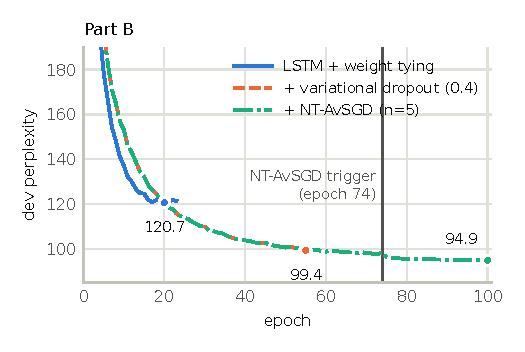
\includegraphics[width=\columnwidth]{figures/lm_dev_ppl.pdf}
  \caption{Dev perplexity of the language models of part B after every epoch; dots mark the selected weights. The two runs
  with variational dropout coincide up to epoch 58, where early stopping ends the one without NT-AvSGD.}
  \label{fig:curves}
\end{figure}



\para{Language modelling.} Every step lowers the perplexity (Table~\ref{tab:lm}). In part A, dropout gains 15.2
test points and AdamW, on the same model, a further 17.0; in part B, variational dropout gives the largest gain of
the study ($-19.5$) and NT-AvSGD a further $-5.1$. The curves of Figure~\ref{fig:curves} show that the last gain
has two sources. Without early stopping before the trigger, SGD keeps improving after epoch 58, where the run
without NT-AvSGD stopped, and reaches 97.6 dev PPL at epoch 72; averaging, triggered at epoch 74, brings it to
94.9. Of the 4.5 dev points gained over variational dropout, 1.8 come from the longer training that the stopping
rule of NT-AvSGD allows and 2.7 from the averaging itself: an ablation that compares the two runs as they are
attributes to averaging about 40\% of a gain that belongs to the training budget.

\begin{table*}[t]
  \caption{Errors of the original implementation, their effect on the reported study and the test that now fails
  if the error comes back (all are verified by mutation, Section~\ref{sec:checks}).}
  \label{tab:errors}
  \centering
  \small
  \setlength{\tabcolsep}{4pt}
  \begin{tabular}{l p{5.2cm} p{5.6cm} p{4.1cm}}
    \toprule
    Class & Error & Effect on the reported study & Caught by \\
    \midrule
    Algorithm & The ``LSTM'' baseline was built with \texttt{nn.RNN} & The 160.0 PPL baseline was a vanilla RNN;
      every later gain of part A was inflated & architecture test \\
    & NT-AvSGD triggered without the non-monotone interval & Averaging started at the first epoch without
      improvement & unit test on a synthetic trace \\
    & NT-AvSGD averaged per-epoch snapshots and selected the SGD weights & The tested weights were never
      validated on dev & running-mean and selection tests \\
    \midrule
    Protocol & The dropout model also tied the input and output embeddings & The dropout step mixed two techniques
      & test on the experiment registry \\
    & AdamW was applied to the model without dropout & The AdamW step did not start from the best model & test on
      the experiment registry \\
    & ATIS models were tested at their last epoch & Test scores of an overfitted model, 15 epochs after the best &
      best-epoch restore test \\
    & Spread as population standard deviation, no significance test & Spread underestimated, differences between
      models untested & sample-std test; Welch's t-test \\
    \midrule
    Dead code & ATIS dropout was applied after the intent logits & The intent layer never saw dropout & behavioural
      test: with $p=1$ the logits are the biases \\
    \midrule
    Determinism & Label ids came from iterating a set of strings & Ids changed from one process to the next &
      sorted-ids test \\
    \midrule
    Infrastructure & Checkpoint folder never created; every run overwrote the checkpoint & No model selected on dev
      was ever saved & end-to-end tests \\
    \midrule
    Lost code & BERT code never committed; labels copied to every sub-token & 89.0 slot F1, the score of a randomly
      initialised BERT & invariance test (lr 0), alignment and oracle tests \\
    \bottomrule
  \end{tabular}
\end{table*}

\para{Intent classification and slot filling.} The bidirectional encoder and BERT bring significant gains on both
tasks (Table~\ref{tab:slu}). Dropout does not: $+0.46$ F1 (95\% CI $[-0.11, +1.04]$, $p=0.10$) and $+0.40$ points
of accuracy ($[-0.02, +0.83]$, $p=0.06$) are within the variation between seeds. Selecting a run is not the same
as measuring a model: the BERT run with the best dev F1, the one kept as checkpoint, has the lowest test F1 of the
five (95.33 against a mean of 95.49).





\section{What the audit changed}
\label{sec:audit}


Table~\ref{tab:errors} lists the errors of the original implementation. For each step we compare the effect it
reported with the effect after the audit (Table~\ref{tab:effects}, Figure~\ref{fig:effects}) with a fixed rule: an
effect whose audited difference is not significant is \emph{not significant}; otherwise the conclusion is
\emph{reversed} if the signs differ, \emph{overstated} or \emph{understated} if the two effects differ by more than
a factor of two, and \emph{confirmed} otherwise. Weight tying is left out: in both studies its baseline is trained
with other hyperparameters.

Seven of the ten effects change. The dropout step of part A is overstated $3.8\times$ because its baseline was a
vanilla RNN (160.0 PPL) and the dropout model also tied the weights: two techniques and a weaker baseline were
credited to dropout. The AdamW step is understated $16\times$ because AdamW was applied to the model without
dropout and compared with the model with dropout and tying. NT-AvSGD reverses sign: the trigger ignored the
non-monotone interval and fired at the first epoch without improvement, the average was taken over per-epoch
snapshots instead of the iterates, and the tested weights were not the ones selected on dev. On ATIS, the
original BERT reached 89.0 slot F1, 5.3 points below the BiLSTM; the audited one is 0.9 points above it. The code
of that run was never committed, but a randomly initialised two-layer BERT trained with our pipeline reaches 88.7,
which suggests that the pre-trained weights were lost, for instance by applying the initialisation of the LSTM
models to every linear layer of BERT. The intent accuracy of the dropout model, which the original study saw fall,
came from a model whose dropout was applied after the intent logits and never reached the intent layer.

None of these errors raised an exception, and every number was in a plausible range. Two were explained away in
the original report, the weak NT-AvSGD result as sensitivity to hyperparameters and the weak BERT result as noise
introduced by WordPiece, and the drop of intent accuracy after dropout was reported as a further gain. A plausible
explanation of an implausible result is the moment an audit should start.

\begin{table}[t]
  \caption{Step-wise effects reported by the original implementation and after the audit (test PPL reduction, or
  gain in points of F1 and accuracy; positive: the step helps).}
  \label{tab:effects}
  \centering
  \footnotesize
  \setlength{\tabcolsep}{3.5pt}
  % Generated by paper/analysis.py from results/: do not edit by hand
\begin{tabular}{l l r r l}
  \toprule
  Step & Metric & Original & Audited & Outcome \\
  \midrule
  + dropout & PPL & +57.6 & +15.2 & 3.8$\times$ overstated \\
  + AdamW & PPL & +1.1 & +17.0 & 16$\times$ understated \\
  + variational dropout & PPL & +22.2 & +19.5 & confirmed \\
  + NT-AvSGD & PPL & -0.2 & +5.1 & sign reversed \\
  \midrule
  BiLSTM & slot F1 & +1.34 & +1.89 & confirmed \\
  BiLSTM & intent acc. & +2.35 & +1.10 & 2.1$\times$ overstated \\
  + dropout & slot F1 & +0.42 & +0.46 & not significant \\
  + dropout & intent acc. & -0.34 & +0.40 & not significant \\
  BERT & slot F1 & -5.32 & +0.90 & sign reversed \\
  BERT & intent acc. & +1.94 & +2.60 & confirmed \\
  \bottomrule
\end{tabular}

\end{table}


\section{Catching the errors}
\label{sec:checks}

The re-implementation is a Python package whose test suite combines five kinds of checks.
\begin{tightlist}
  \item \textbf{Oracle evaluation.} A fake model that returns the gold labels must score exactly 1.0, for the LSTM
    models and for BERT: the cheapest way to trust a metric.
  \item \textbf{Tests from the definition.} The NT-AvSGD trigger on a synthetic trace, its running mean against the
    mean of the iterates, the variational mask constant over time, dropout that zeroes the inputs of both output
    layers when $p=1$.
  \item \textbf{Invariance.} Trained with a learning rate of 0, BERT must save exactly its pre-trained encoder;
    anything that re-initialises weights during training breaks the equality.
  \item \textbf{Protocol.} Consecutive experiments must differ only in the keys of the technique they add; the
    best dev epoch, not the last, must be the one left in the model.
  \item \textbf{End-to-end.} Both command lines train for a few epochs, save a checkpoint, reload it and must
    reproduce the recorded scores.
\end{tightlist}
To measure the suite we re-introduce each error of Table~\ref{tab:errors} that can be written as a code change
(12 mutants), the suspected cause of the BERT result, and three plausible variants of the same errors in other
places (testing the language models on their last epoch, re-initialising the weights at every epoch, keeping a
reference to the best weights instead of a copy). The suite kills all 16 mutants. Mutation analysis also tested
the tests: in its first run, two mutants of the language-model training survived, and the tests that now kill
them were written because of it. The suite runs in 45 seconds on a CPU and the mutation analysis in two and a half
minutes; both run on every push.

\section{Limitations}

The audit covers one study, and its author also wrote the original implementation: the errors are the ones the
tests can see, not necessarily all of them. The two implementations also differ in some hyperparameters, so
Table~\ref{tab:effects} measures the combined effect of fixes and changes. The language models were trained with
a single seed, so their effects have no confidence interval, and the original numbers come from reports whose BERT
code is lost. The mutants are known errors: killing them shows that the suite guards against these errors, not
against unknown ones.

\section{Conclusion}

Seven of the ten conclusions of the original study changed after the audit, and nothing in its numbers signalled
it. The errors were ordinary: a wrong class name, a confounded configuration, a misread stopping rule, a dropout in
the wrong line. The checks that catch them are cheap, and most follow from treating each ablation step as a claim:
a configuration diff that shows one change, an effect reported with its spread and a significance test, and a test
that fails if the technique is silently disabled.

{\footnotesize
\setlength{\bibsep}{0.6pt plus 0.3pt}
\bibliographystyle{plainnat}
\bibliography{references}
}

\end{document}
